% Options for packages loaded elsewhere
\PassOptionsToPackage{unicode}{hyperref}
\PassOptionsToPackage{hyphens}{url}
\PassOptionsToPackage{dvipsnames,svgnames,x11names}{xcolor}
%
\documentclass[
  12pt,
  letterpaper,
]{article}

\usepackage{amsmath,amssymb}
\usepackage{iftex}
\ifPDFTeX
  \usepackage[T1]{fontenc}
  \usepackage[utf8]{inputenc}
  \usepackage{textcomp} % provide euro and other symbols
\else % if luatex or xetex
  \usepackage{unicode-math}
  \defaultfontfeatures{Scale=MatchLowercase}
  \defaultfontfeatures[\rmfamily]{Ligatures=TeX,Scale=1}
\fi
\usepackage{lmodern}
\ifPDFTeX\else  
    % xetex/luatex font selection
  \setmainfont[]{Baskerville}
  \setsansfont[]{Futura}
\fi
% Use upquote if available, for straight quotes in verbatim environments
\IfFileExists{upquote.sty}{\usepackage{upquote}}{}
\IfFileExists{microtype.sty}{% use microtype if available
  \usepackage[]{microtype}
  \UseMicrotypeSet[protrusion]{basicmath} % disable protrusion for tt fonts
}{}
\makeatletter
\@ifundefined{KOMAClassName}{% if non-KOMA class
  \IfFileExists{parskip.sty}{%
    \usepackage{parskip}
  }{% else
    \setlength{\parindent}{0pt}
    \setlength{\parskip}{6pt plus 2pt minus 1pt}}
}{% if KOMA class
  \KOMAoptions{parskip=half}}
\makeatother
\usepackage{xcolor}
\usepackage[margin=1in]{geometry}
\setlength{\emergencystretch}{3em} % prevent overfull lines
\setcounter{secnumdepth}{-\maxdimen} % remove section numbering


\providecommand{\tightlist}{%
  \setlength{\itemsep}{0pt}\setlength{\parskip}{0pt}}\usepackage{longtable,booktabs,array}
\usepackage{calc} % for calculating minipage widths
% Correct order of tables after \paragraph or \subparagraph
\usepackage{etoolbox}
\makeatletter
\patchcmd\longtable{\par}{\if@noskipsec\mbox{}\fi\par}{}{}
\makeatother
% Allow footnotes in longtable head/foot
\IfFileExists{footnotehyper.sty}{\usepackage{footnotehyper}}{\usepackage{footnote}}
\makesavenoteenv{longtable}
\usepackage{graphicx}
\makeatletter
\def\maxwidth{\ifdim\Gin@nat@width>\linewidth\linewidth\else\Gin@nat@width\fi}
\def\maxheight{\ifdim\Gin@nat@height>\textheight\textheight\else\Gin@nat@height\fi}
\makeatother
% Scale images if necessary, so that they will not overflow the page
% margins by default, and it is still possible to overwrite the defaults
% using explicit options in \includegraphics[width, height, ...]{}
\setkeys{Gin}{width=\maxwidth,height=\maxheight,keepaspectratio}
% Set default figure placement to htbp
\makeatletter
\def\fps@figure{htbp}
\makeatother
\newlength{\cslhangindent}
\setlength{\cslhangindent}{1.5em}
\newlength{\csllabelwidth}
\setlength{\csllabelwidth}{3em}
\newlength{\cslentryspacingunit} % times entry-spacing
\setlength{\cslentryspacingunit}{\parskip}
\newenvironment{CSLReferences}[2] % #1 hanging-ident, #2 entry spacing
 {% don't indent paragraphs
  \setlength{\parindent}{0pt}
  % turn on hanging indent if param 1 is 1
  \ifodd #1
  \let\oldpar\par
  \def\par{\hangindent=\cslhangindent\oldpar}
  \fi
  % set entry spacing
  \setlength{\parskip}{#2\cslentryspacingunit}
 }%
 {}
\usepackage{calc}
\newcommand{\CSLBlock}[1]{#1\hfill\break}
\newcommand{\CSLLeftMargin}[1]{\parbox[t]{\csllabelwidth}{#1}}
\newcommand{\CSLRightInline}[1]{\parbox[t]{\linewidth - \csllabelwidth}{#1}\break}
\newcommand{\CSLIndent}[1]{\hspace{\cslhangindent}#1}

% -----------------------
% CUSTOM PREAMBLE STUFF
% -----------------------

% -----------------
% Title block stuff
% -----------------

% Abstract
\usepackage[runin]{abstract}
\renewcommand{\abstractnamefont}{\sffamily\small\bfseries}
\renewcommand{\abstracttextfont}{\sffamily\small}
\setlength{\absleftindent}{5pt}
\setlength{\absrightindent}{\absleftindent}

% Title
\usepackage{titling}
\pretitle{\par\begin{flushleft}\LARGE\sffamily\bfseries}
\posttitle{\par\end{flushleft}\vskip 10pt}

% Keywords
\newenvironment{keywords}
{\small\sffamily{\sffamily\small\bfseries{Keywords.}}}

% Authors
\usepackage{orcidlink}  % Create automatic ORCID icons/links
%\renewcommand{\and}{\end{tabular} \hskip 3em \begin{tabular}[t]{@{\hspace{0em}}l@{}}}
\preauthor{\begin{flushleft}
           \lineskip 1.5em}
\postauthor{\end{flushleft}}

% ------------------
% Section headings
% ------------------
\usepackage{titlesec}
\titleformat*{\section}{\Large\sffamily\bfseries\raggedright}
\titleformat*{\subsection}{\large\sffamily\bfseries\raggedright}
\titleformat*{\subsubsection}{\normalsize\sffamily\bfseries\raggedright}
\titleformat*{\paragraph}{\small\sffamily\bfseries\raggedright}

%\titlespacing{<command>}{<left>}{<before-sep>}{<after-sep>}
% Starred version removes indentation in following paragraph
\titlespacing*{\section}{0em}{2em}{0.1em}
\titlespacing*{\subsection}{0em}{1.25em}{0.1em}
\titlespacing*{\subsubsection}{0em}{0.75em}{0em}

% ------------------
% Headers/Footers
% ------------------
\usepackage{fancyhdr}
\pagestyle{fancy}
\fancyhf{}
\fancyhead[L,C]{}
\fancyhead[R]{\leftmark}
\fancyfoot[L,C]{}
\fancyfoot[R]{\thepage}
\renewcommand{\headrulewidth}{1pt}
\fancypagestyle{plain}{%
    \renewcommand{\headrulewidth}{0pt}%
    \fancyhf{}%
    \fancyfoot[R]{\thepage}%
}
\renewcommand\footnoterule{\rule{\linewidth}{0.1pt}\vspace{5pt}}

% ------------------
% Captions
% ------------------
\usepackage[labelfont=bf,labelsep=period]{caption}
\captionsetup[figure]{font=footnotesize,justification=raggedright,singlelinecheck=false,format=hang}


% ---------------------------
% END CUSTOM PREAMBLE STUFF
% ---------------------------
\usepackage{dcolumn}
\makeatletter
\makeatother
\makeatletter
\makeatother
\makeatletter
\@ifpackageloaded{caption}{}{\usepackage{caption}}
\AtBeginDocument{%
\ifdefined\contentsname
  \renewcommand*\contentsname{Table of contents}
\else
  \newcommand\contentsname{Table of contents}
\fi
\ifdefined\listfigurename
  \renewcommand*\listfigurename{List of Figures}
\else
  \newcommand\listfigurename{List of Figures}
\fi
\ifdefined\listtablename
  \renewcommand*\listtablename{List of Tables}
\else
  \newcommand\listtablename{List of Tables}
\fi
\ifdefined\figurename
  \renewcommand*\figurename{Figure}
\else
  \newcommand\figurename{Figure}
\fi
\ifdefined\tablename
  \renewcommand*\tablename{Table}
\else
  \newcommand\tablename{Table}
\fi
}
\@ifpackageloaded{float}{}{\usepackage{float}}
\floatstyle{ruled}
\@ifundefined{c@chapter}{\newfloat{codelisting}{h}{lop}}{\newfloat{codelisting}{h}{lop}[chapter]}
\floatname{codelisting}{Listing}
\newcommand*\listoflistings{\listof{codelisting}{List of Listings}}
\makeatother
\makeatletter
\@ifpackageloaded{caption}{}{\usepackage{caption}}
\@ifpackageloaded{subcaption}{}{\usepackage{subcaption}}
\makeatother
\makeatletter
\@ifpackageloaded{tcolorbox}{}{\usepackage[skins,breakable]{tcolorbox}}
\makeatother
\makeatletter
\@ifundefined{shadecolor}{\definecolor{shadecolor}{rgb}{.97, .97, .97}}
\makeatother
\makeatletter
\makeatother
\makeatletter
\makeatother
\ifLuaTeX
  \usepackage{selnolig}  % disable illegal ligatures
\fi
\IfFileExists{bookmark.sty}{\usepackage{bookmark}}{\usepackage{hyperref}}
\IfFileExists{xurl.sty}{\usepackage{xurl}}{} % add URL line breaks if available
\urlstyle{same} % disable monospaced font for URLs
\hypersetup{
  pdftitle={Religiosity as Influenced by Intersectionality},
  pdfauthor={Kevin Gable},
  pdfkeywords={keyword1, keyword2},
  colorlinks=true,
  linkcolor={blue},
  filecolor={Maroon},
  citecolor={Blue},
  urlcolor={red},
  pdfcreator={LaTeX via pandoc}}


\title{Religiosity as Influenced by Intersectionality\thanks{Thanks to
everyone for checking this out.}}
% subtitles do not seem to work with article class?
%%\subtitle{}

\author{
{\bfseries \normalsize Kevin Gable}%
\thanks{Corresponding author.} \\%
 \small University of Oregon, Sociology \\%
{\footnotesize \url{kgable@uoregon.edu}} \\\vspace{10pt}
}

\predate{}
\postdate{}
\date{}
\begin{document}

% for some reason this does not work in header
\renewcommand{\abstractname}{Abstract.}

\fancyhead[L]{Paper}

% need to redefine this environment to get enough spacing of 
% bibliography after title
\renewenvironment{CSLReferences}[2] % #1 hanging-ident, #2 entry spacing
 {% don't indent paragraphs
  \vspace{10pt}
  \setlength{\parindent}{0pt}
  % turn on hanging indent if param 1 is 1
  \ifodd #1
  \let\oldpar\par
  \def\par{\hangindent=\cslhangindent\oldpar}
  \fi
  % set entry spacing
  \setlength{\parskip}{#2\cslentryspacingunit}
 }%
 {}

\maketitle
%\noindent \rule{\linewidth}{.5pt}
\begin{abstract}
An Abstract
\end{abstract}
\begin{keywords}
\def\sep{;\ }
keyword1\sep 
keyword2
\end{keywords}
%\noindent \rule{\linewidth}{.5pt}
\ifdefined\Shaded\renewenvironment{Shaded}{\begin{tcolorbox}[boxrule=0pt, breakable, enhanced, frame hidden, borderline west={3pt}{0pt}{shadecolor}, sharp corners, interior hidden]}{\end{tcolorbox}}\fi

\hypertarget{introduction}{%
\section{Introduction}\label{introduction}}

Religious belief is an important component of social construction. The
United States provides an interesting area to study trends in religious
beliefs. The religious freedom in the United States has brought together
a wide range of religious institutions, beliefs, and practices including
no belief at all. However, these beliefs are not created and do not
exist in a vacuum. Each component of society interacts with religious
belief and vice-versa. For example, education, gender, race,
socioeconomic status, and age are all factors both influencing religious
belief and being influenced by religious belief and practices. The
opportunity of religious freedom allows for each aspect of the human
experience to influence and be influenced by trends in religiosity.

Intersectionality is referred to in sociology as the interconnected
nature of social categorizations such gender, race, and class creating
overlapping and independent systems of advantage or disadvantage.
Religiosity is a term describing the importance of and influence
religious beliefs and practices have on individuals and society. We have
seen in the United States changes in trends in religiosity over time.
These changes are likely influenced by the interconnecting aspects of
human identity. Previous studies have shown negative associations
between levels of education and religiosity over time. Some studies have
shown age having a positive influence on religiosity over time as well.
Other studies have shown international results highlighting a negative
association between religious importance and GDP as a socioeconomic
factor, but found education to be a mediator. Some research has shown
women to be more religious than men, on average, when considering
intrinsic measure of religious importance and daily spiritual
experiences. Other research has even shown interesting similatrities
between the religiously affiliated and unaffiliated in the United
States.

There are measurable trends in religious and spiritual beliefs and
practices over the last century and they give rise to some interesting
questions. What societal factors influence the change in religious and
spiritual beliefs? How does this potentially change with age and between
generations? How do these aspects work together to influence a persons
measurable religiosity?

\hypertarget{background}{%
\section{Background}\label{background}}

One of the reasons much research has been done in this area is the
social meaning of religious and spiritual beliefs are important and
change over time. The social meaning is important because meaning itself
is not a static or stable monolith. It circulates through society and
changes over time. Meaning is intrinsically on the move and can be
understood as effect of signs and symbols and is tied to cognitive and
environmental motivation. Cognitive motivation includes the aspects of
culture an individual has internalized. Environmental motivation likely
motivates meaning as well. Therefore, motivation arises from the ongoing
interaction between the individual and the environment. (Norton 2018)
Dr.~Norton creates a useful pragmatist view of the meaning identifying
three categories; ``What matters?'', ``What are you going to do about
it?'', and ``Why?'' As members of society we draw from our experiences
through intersectionality to answer these questions. It is additionally
interesting when considering the social meaning of something as old in
human history as religious and spiritual meaning due to the temporal
aspect of meaning.

Allowing meaning as a concept to shift to an occurrence in the mind
and/or environment allows meaning to become a processual category and it
suggests meaning manifests as actions, events, ideas, habits,
dispositions, and even more collections of signs and social
regularities. (Norton 2018) The trends in religious and spiritual
beliefs may be tied to this phenomenon of meaning on the move and its
interactions between individuals and their environment. As the social
and educational landscapes of the United States changed over the last
century, so did the social meaning of religious/spiritual beliefs and
practices. These changes may be measured through analyzing associations
between trends in religiosity, educational factors, and social factors
over time. Existing trends in previous research provides interesting
clues and questions.

A study examining GSS data from 1972-2016, found interesting trends in
the beliefs and practices of the religiously affiliated and the
unaffiliated in the United States. From 1973 to 2000, belief in the
afterlife increased for both the religiously affiliated and the
unaffiliated. However, a clear divergence emerges in the year 2000. The
belief in the afterlife for the affiliated increased while it decreased
for the unaffiliated. This same trend was found in the belief in God.
(Gullickson 2018) Dr.~Gullickson explains the population of the
unaffiliated is composed of those who were never affiliated and those
who are disaffiliated and adds after the year 2000, the population of
the never affiliated seemed to level off in terms of growth. However,
the population of the disaffiliated grew substantially. This divergence
is interesting. Is this shift associated with the social meaning of
religious/spiritual beliefs and practices on the move as interacting
between individuals and their environment? If so how and what factors of
intersectionality are potentially involved? Care must be utilized when
measuring these associations. Correlation does not mean causation.
However, understanding more about how the intersecting aspects of human
social identity influences how meaning moves may provide clues on how
other areas of social construction changes over time as well.

In a study involving 626 participants, the influence of education, sex,
and age on religiosity was conducted. The results were examined across
three cohorts, the Baby Boomer generation, Generation X, and Generation
Y. Results showed females in the Baby Boomer and Generation X scored
higher on the intrinsic religiosity than males. A positive relation was
found between education and both daily spiritual experiences and
intrinsic religiosity with a negative relation found between education
and extrinsic religiosity. Additionally, Generation Y reported higher
levels of extrinsic religiosity and Generation Y females socred lower on
daily spiritual experiences and intrinsic religiosity than males.
(\textbf{Green2013?}) This is interesting because this observed pattern
seems similar to the divergence noted between the religiously affiliated
and unaffiliated in Dr.~Gullickon's research. Education and gender are
not the only intersecting factor either.

AN international study of religiosity and education found interesting
associations with GDP. When considering the process of modernization,
researchers postulated the objective of modernization is economic growth
and is adjacent to a secularization process. However, when examining the
relation between education and religiosity it was found education served
as a mediator between religiosity and GDP. This may account for some of
the variation found between countries as some have religion more heavily
integrated into education. (\textbf{Ha2019?}) The level of integration
between religion and education would likely produce different results.
If the social meaning of religiosity itself is the result of cognitive
and environmental motivaiton we shold expect to see differing results
from the influence of modernization on religious/spiritual beliefs and
practices. Individuals in different social environments will have
different motivations when utilizing the three categories of meaning.
This is the importance of intersectionality in constructing social
meaning while also allowing it to move through both groups and time.

A longitudinal analysis of the effects of higher education on
religiosity found a decline in religiosity upon achieving a Bachelors
degree. The same study also found an increase in religiosity scores
among respondents as they aged. through adulthood. This implies two
things. First, people may become less religious as they enter college
and leave direct parental influence. This may be influenced by social
and academic curriculum. Second, this implies after earning a Bachelors
degree and moving tthrough adult life, the process of starting a family
may influence religious patterns among aging adults in a positive
relationship. (\emph{Does Higher Education Cause Religious Decline?: A
Longitudinal Analysis of the Within- and Between- Person Effects of
Higher Education on Religiosity.} 2016) However, it should also be noted
in another study examining the cross-national effects of higher
education on religiosity, it was found GDP served as a mediator between
national-level education and national-level
religiosity(\textbf{Shwadel2015?}) This suggests age has a distinctive
influence on religiosity as well as the social and academic environment
of college. Once again different aspects of human social identity
potentially intersect to facilitate the convergence between cognitive
and environmental motivations allowing the social meaning of
religious/spiritual beliefs and practices to change over time.

The social meaning of religious/spiritual beliefs and practices are
influenced by intersectionality because they are areas of convergence
between cognitive and environmental motivations. This allows the meaning
to change over time as both a person and a society change over time. The
United States provides an interesting population to study the potential
evolution of the social meaning of religious and spiritual importance
due to the diverse religious affiliations, large-scale educational
access, and diverse cultural backgrounds. The question of interest to
this research is, how does the intersections of educational attainment
and racial identification potentially influence religiosity? Given the
consideration of the previous areas of research mentioned, three main
hypothesis emerge. First, as educational attainment increases,
religiosity will decrease. If there is an environmental motivation
factor influencing religiosity and it is observed to decrease upon
entering college, religiosity should decrease as education continues.
Second, because all groups in the United States do not experience the
same access to the large-scale educational system, differences should be
seen in religiosity among educational attainment across racial
categories. Third, because these factors intersect with the specific
religion with which a respondent is affiliated, (or even in the case
where that religion is none) differences in religiosity scores should be
seen across educational attainment and racial identification when
controlling for religious affiliation.

\hypertarget{data-and-methods}{%
\section{Data and Methods}\label{data-and-methods}}

This research project utilizes a repeated cross-sectional study design
focusing on GSS (General Social Survey) data from 2006 to 2018. These
years were chosen for the availability of data concerning questions used
to construct a measure of religiosity. The questions used to construct a
measure of religiosity are frequency of service attendance, frequency of
prayer, respondent's belief in God, and how important is religion to the
individual respondent. Service attendance is recorded as an ordinal
variable with the following categories; never, yearly, monthly, weekly,
and more than weekly. Frequency of prayer is recorded as an ordinal
variable with the following categories; never, weekly, daily, more than
daily. The respondent's belief in God is recorded as an ordinal variable
with the following categories; no belief, belief in a higher power,
belief but doubts, and believes with no doubt. The measure of religious
importance to the individual respondent is recorded as an ordinal
variable with the following categories; no religion, not strong,
somewhat strong, and strong. These variables were used in a summated
scale to create the overall measure of religiosity.

Educational attainment among respondents was collapsed into the
following categories; less than high school, high school, some college
(including trade certifications and associate degrees), bachelors
degree, and graduate degree (including masters degrees and PhD's). The
racial identification of respondents were collapsed into the following
categories; white, black, latinx, asian, and asian/pacific islander. In
order to control for religious affiliation, the following categories of
affiliation were considered; Protestant, Catholic, Other Christian
(which includes the categories ``Christian'', ``Orthodox Christian'',
and ``Inter-nondenominational''), Jewish, Muslim, Buddhist, Hindu,
other, (which includes Indigenous and other Eastern religions) and none.
In order to consider the temporal intersection, age was both kept as a
quantitative variable and collapsed in ten-year-age groups with the
exception of the first age group, 18-29. This group was constructed due
to a small amount of respondents in the 18-19 year-old age group.
Respondent's gender was recorded as male or female as that is the format
of the GSS. Cases with missing data were dropped to allow for a
complete-case analysis of the remaining observations. All models were
created as general linear models. However, the age squared term in
models one through four control for the non-linear effects of age.

\hypertarget{limitations}{%
\section{Limitations}\label{limitations}}

There are several limitations to consider in this research. First,
correlation is not causation. Even potentially finding relationships
between religiosity, education, and race does not mean education and/or
race ``cause'' an effect. There can be a measure of association, but
likely other factors contribute as well. Due to the nature of
intersectionality, it is likely numerous intersections play a role. This
research project is only limited to examining the potential association
between the identified variables. Second, race itself is not a physical
category, it is a social construction. This means any influence or
association is not the result of some biological factor and more likley
associated with cultural factors for both the individual group and the
influence of the larger collective. Finally, the very measure of
religiosity may be flawed in that it does not consistently measure the
individual variables used to create religiosity across all religions.
This may lead to systematic under of over counting with consideration of
these intersections.

\hypertarget{potential-issues-in-measuring-religiosity}{%
\section{Potential Issues in Measuring
Religiosity}\label{potential-issues-in-measuring-religiosity}}

There are two specific areas of interest when identifying the
limitations of this study; religious attendance and the belief in God of
each respondent. This must be aknowleged because these are two of the
four categories used to construct the religiosity measure. More so, they
are ordinal variables and therefore have a value rating in a specific
order. There is no set specific measure of religiosity. However, the
four selected for this research are four of the most commonly used
categories.

Measuring religious attendance was done by asking respondents how often
they attended religious service. The given options to respond were;
never, yearly, monthly, weekly, and more than weekly. This means a
respondent attending service at a weekly rate will score higher in the
service attendance category than a respondent who indicates they attend
monthly. This works fine as long as each religion and each intersection
is measured equaly. However, each religion and each culture has slight
differences in practices and beliefs.

\begin{figure}[!t]

{\centering 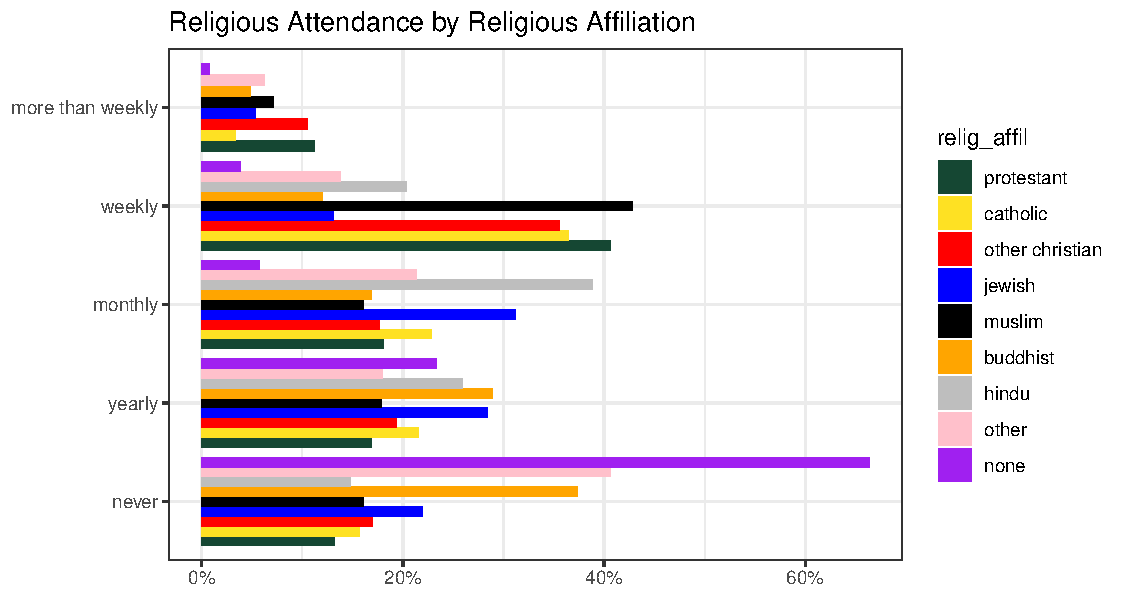
\includegraphics{main_manuscript_files/figure-pdf/fig-Religious_Attendance_by_Religious_Affiliation-1.pdf}

}

\caption{\label{fig-Religious_Attendance_by_Religious_Affiliation}Religious
Attendance by Religious Affiliation}

\end{figure}

As seen in
Figure~\ref{fig-Religious_Attendance_by_Religious_Affiliation} there are
two categories highly represented as never attending service; ``other'',
and ``Buddhist''. This can be problematic as service requirements and
structure may not be the same for these two groups as they are for the
other represented affiliations. Because this is an ordinal variable
contributing it's score to the overall religiosity measure, these two
groups may be systematically under-considered. The ``other'' category
includes indigenous and other eastern religions. It could be problematic
to value their service attendance rating in this manner. If a religion
does not have within it's structure a need to go to a specific service
at a specific time, it potentially underscores the actual religiosity of
those in that group. It also prioritizes the Christian religious format
because service attendance is, on average, a large part of that
religious practice. This is not the only potential issue with using
religious attendance as a variable to create a measure of religiosity.
There are differences across gender as well.

\begin{figure}[!t]

{\centering 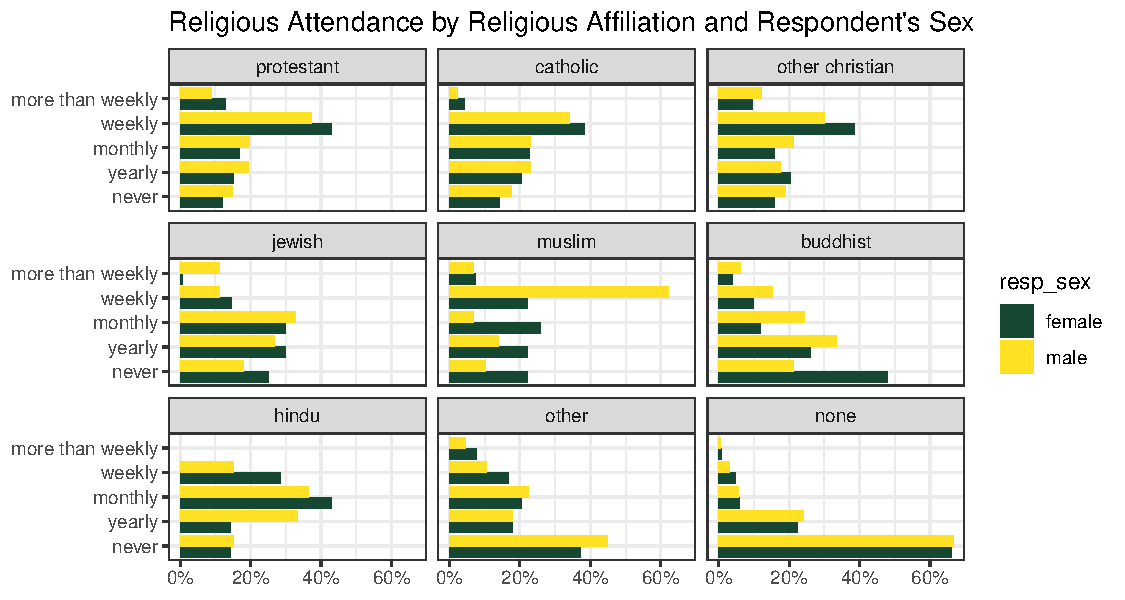
\includegraphics{main_manuscript_files/figure-pdf/fig-Religious_Attendance_by_Respondents_Sex_and_Religious_Affilation-1.pdf}

}

\caption{\label{fig-Religious_Attendance_by_Respondents_Sex_and_Religious_Affilation}Religious
Attendence by Respondents Sex and Religious Affiliation}

\end{figure}

As shown in
Figure~\ref{fig-Religious_Attendance_by_Respondents_Sex_and_Religious_Affilation}
it is seen men and women do not all have the same service attendance
habits across religions. For example, within the Muslim faith it can be
seen men attend service more often than women. This is most noticeable
in the ``weekly'' category for attendance. Within this category, men are
over represented compared to women. There are likely cultural
explanations for this difference in service attendance. This difference
in attendance needs to be considered when using attendance as a
composite in the religiosity variable. Additionally, The Buddhist faith
seems to show a similar pattern. Women are over represented in the
``never'' category while men are the majority in each other category.
Again, there is likely a systematic misrepresentation of attendance
based on gender factors.

In the case of religious attendance used as a composite measure of
religiosity there may be concern for misrepresentation in religious
importance. Differences in attendance resulting from cultural structures
or the service structure of particular religions do not necessarily mean
one group is more or less religious than another. It simply means there
are cultural or structural differences in how a religion is integrated
into a particular society. This is not the only potential issue. Belief
in god could also be considered in this way.

\begin{figure}[!t]

{\centering 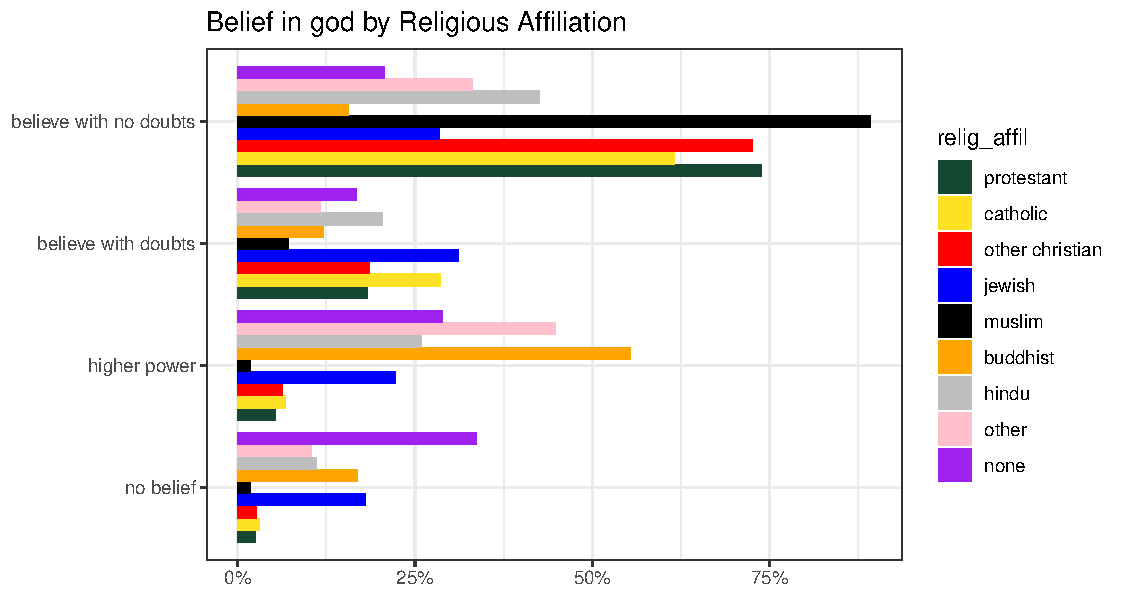
\includegraphics{main_manuscript_files/figure-pdf/fig-Beleif_in_God_by_Religious_Affiliation-1.pdf}

}

\caption{\label{fig-Beleif_in_God_by_Religious_Affiliation}Belief in God
of Respondents by Religious Afiliation.}

\end{figure}

As shown in Figure~\ref{fig-Beleif_in_God_by_Religious_Affiliation} it
is seen Buddhists are the majority representation in the belief in a
higher power. However, this could be an issue because it implies a
belief in a higher power is less religious than a belief in a god. This
is an ordinal variable giving more value to the answers professing a
belief in a specific god. as with service attendance, the ``other''
category must also be considered. It may be problematic to place
indigenous beliefs below Christian because they do not incorporate the
same or a single deity belief system. That, in and of itself, is not
enough to classify them as less religious.

In each of these cases it is problematic to use the current, and most
commonly used, measures of religiosity. They seem to prioritize
Christian religious beliefs and practices. This may not give us a
measure of religiosity usable across religious affiliations or gender.
This project utilized 4 of the 5 most common variables used to create a
measure of religiosity. If two variables potentially have issues with
under or over representing certain groups due to cultural or religious
structural reasons, the overall measure should contain a rather large
margin of error preventing accurate predictions of associations. It may
be best to consider options allowing the measure of religiosity to be
done within religions instead of across them. This would require
internal considerations for each affiliation to account for cultural and
structural differences, then using internal measures to create an
overall religiosity applicable to specific religious/spiritual belief
systems. This could potentially provide a more robust analysis of
aggregate religiosity. Meaning is on the move and it is seen in these
examples. As the social meaning of religious/spiritual beliefs and
practices moves through society it is incorporated differently depending
on the intersections of human social identity. We can potentially get a
better measure and understanding of this process in the context of
religious structures by comparing the accurate differences and
similarities between them. But, when considering the value or importance
of a respondent's religion, we need to consider the differences more
carefully and work to place the right context on them.

\hypertarget{results}{%
\section{Results}\label{results}}

The focus of this research is to examine the possible associations
between religiosity, education, and racial identification. There are
three main hypothesis postulated. First, as educational attainment
increases, religiosity will decrease. Second, because all groups in the
United States do not experience the same access to the large-scale
educational system, differences should be seen in religiosity among
educational attainment across racial categories. Third, because these
factors intersect with the specific religion with which a respondent is
affiliated, differences in religiosity scores should be seen across
educational attainment and racial identification when controlling for
religious affiliation. These differences may reflect the process of
meaning on the move. As each group in the United States integrates their
social identity they go through the process of integrating the three
categories of the pragmatist view of meaning; ``What matters?'', ``What
are you going to do about it?'', and ``Why?'' During this process, each
intersection of human social identity comes into play creating the
foundation for both internalizing the social meaning of
religious/spiritual beliefs and practices. Here, both the cognitive and
environmental motivations are potentially observed. The process of
internalizing the social meaning of religious/spiritual beliefs and
practices happens at a cognitive level. The intersectional aspect of
human social identity provides a social environmental consideration.
This does not mean physical environments do not have an influence.
Rather, the focus on this research is to observe trends potentially
associated with the intersectionality contribution as it relates to
education and racial identification and it's influence on religiosity.
It is good to begin looking at religiosity across the distribution of
educational attainment.

\begin{figure}[!t]

{\centering 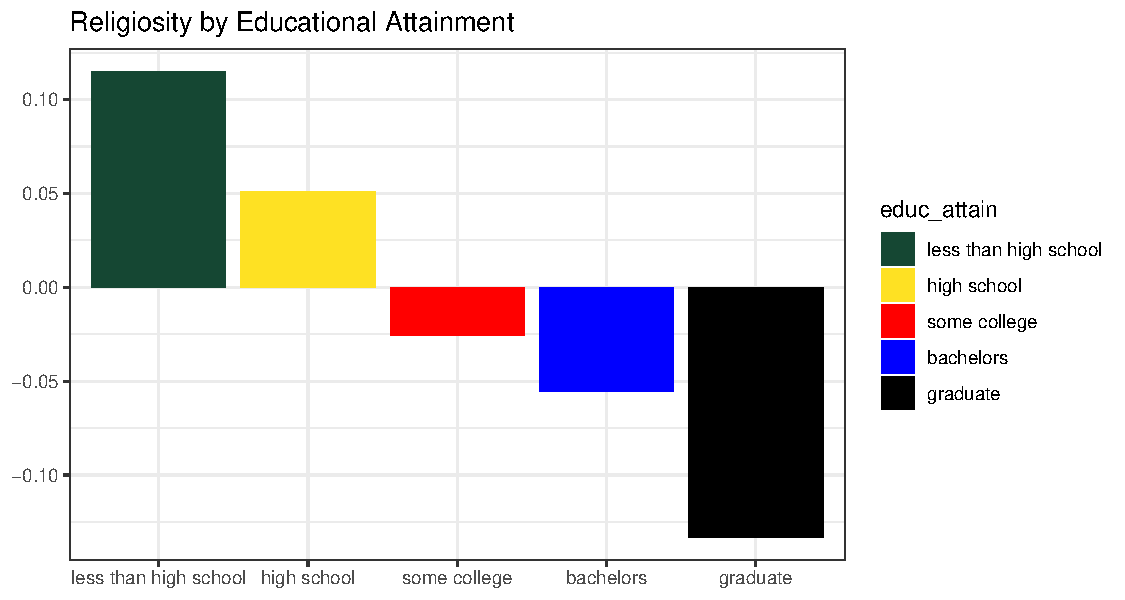
\includegraphics{main_manuscript_files/figure-pdf/unnamed-chunk-5-1.pdf}

}

\caption{Religiousity by Repsondents Educational Attainment}

\end{figure}

When examining the relation between the religiosity and educational
attainment among respondents, the results appear to support hypothesis
one. As seen in \textbf{?@fig-Religiousity\_by\_Educational\_Attainment}
religiosity scores decrease as educational attainment increases. This is
of interest because it may suggest a social environment in education
facilitating the negative relationship with religiosity. However,
caution is needed as correlation is not causation. There are many
factors to consider within educational attainment as previously
mentioned. Each group in the United States has varying access to
different levels of educational attainment. An examination of
eduacational attainment across racial categories will be helpful in
observing trends within the context of intersectionality.

\begin{figure}[!t]

{\centering 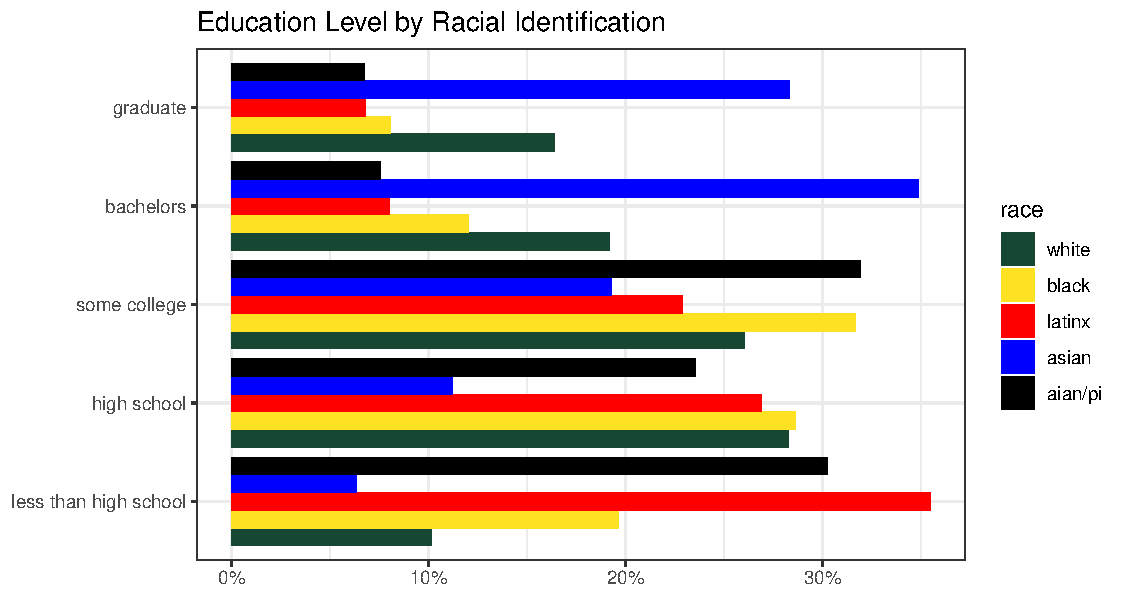
\includegraphics{main_manuscript_files/figure-pdf/fig-Educational_Attainment_by_Race-1.pdf}

}

\caption{\label{fig-Educational_Attainment_by_Race}Level of Educational
Attainment of Respondents by Racial Identification.}

\end{figure}

There are some trends to note when examining the association between
educational attainment and racial identification.As shown in
Figure~\ref{fig-Educational_Attainment_by_Race} educational attainment
varies across racial identification. The Asian and White racial
categories are among the most represented in the educational categories
of bachelors and graduate degrees. The Black and Asian/Pacific Islander
categories represent the majority withing he some college categories.
The Black and White represent the majority in the high school category.
Finally, the latinX group represents the majority in the less than high
school category. There are clear differences in educational attainment
across racial identifications. This is helpful as it relates to the
foundation of hypothesis two. Different racial groups have differing
access to educational attainment. This should produce differences in
religiosity among educational attainment across racial categories. In
terms of intersectionality, a respondents religiosity should be
influenced by the intersection of their racial identification and
specific educational attainment.

\begin{figure}[!t]

{\centering 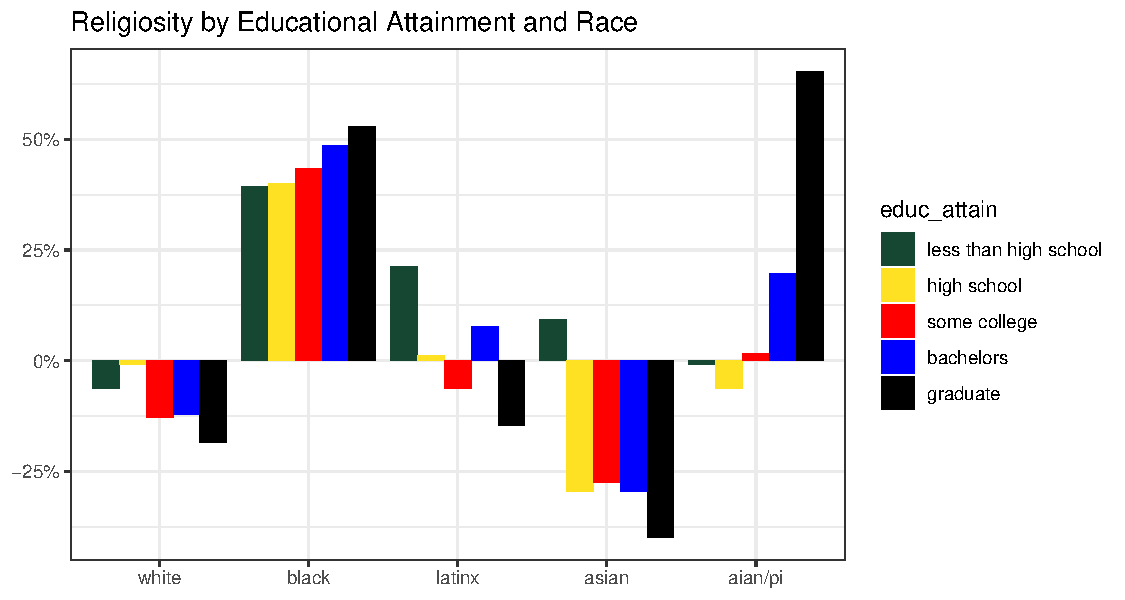
\includegraphics{main_manuscript_files/figure-pdf/unnamed-chunk-7-1.pdf}

}

\caption{Religiousity by Repsondents Education Level and Race}

\end{figure}

Trends begin to emerge when examining religiosity across educational
attainment and racial identification. As shown in
\textbf{?@fig-Religiosity\_by\_Education\_and\_Race} there are clear
differences in religiosity across both factors. This seems to support
hypothesis two. Among the White racial group, religiosity appears to
decrease as educational attainment increases. A similar pattern seems to
emerge for the Asian racial category. The LatinX racial group seems is
of interest because it appears religiosity in that group may not be
influenced by the intersection of educational attainment and racial
identification as much as the other groups. The Black racial category
appears to have the opposite relation than that of Whites and Asians. As
educational attainment increases religiosity also increases. This is an
interesting results. To better understand some of the trend among Black
respondents in this context
Table\_of\_Religiosity\_by\_Education\_and\_Race it appears the trend
may be driven by those not affiliated with a religious group become more
religious as they attain education, on average. Graphs and tables help
to understand some trends. However, in this context, they are more
helpful in defining the questions related to the hypothesis presented.
To better understand, models are needed.

\begin{verbatim}
, ,  = white

                 
                  less than high school high school some college bachelors
  protestant                       57.4        55.3         49.0      46.5
  catholic                         15.6        22.7         21.2      24.2
  other christian                   4.5         3.4          4.1       2.3
  jewish                            0.5         1.0          1.8       3.9
  muslim                            0.0         0.1          0.2       0.3
  buddhist                          0.2         0.3          0.4       0.6
  hindu                             0.0         0.0          0.0       0.1
  other                             1.1         0.7          1.3       0.9
  none                             20.7        16.5         21.9      21.3
                 
                  graduate
  protestant          45.6
  catholic            20.9
  other christian      2.6
  jewish               5.0
  muslim               0.2
  buddhist             0.8
  hindu                0.0
  other                0.9
  none                24.0

, ,  = black

                 
                  less than high school high school some college bachelors
  protestant                       71.2        72.3         70.7      74.5
  catholic                          6.2         5.8          5.5       7.5
  other christian                   2.9         4.4          6.0       4.7
  jewish                            0.5         0.3          0.6       0.0
  muslim                            1.0         0.8          1.2       0.8
  buddhist                          0.0         0.2          0.0       0.0
  hindu                             0.0         0.0          0.0       0.0
  other                             0.5         0.2          0.3       0.4
  none                             17.8        16.0         15.8      12.2
                 
                  graduate
  protestant          73.1
  catholic             8.8
  other christian      6.4
  jewish               0.0
  muslim               0.0
  buddhist             0.0
  hindu                0.0
  other                0.0
  none                11.7

, ,  = latinx

                 
                  less than high school high school some college bachelors
  protestant                       23.6        21.4         21.1      23.0
  catholic                         61.7        55.9         52.2      54.6
  other christian                   2.8         5.6          4.4       2.9
  jewish                            0.0         0.0          0.4       0.6
  muslim                            0.0         0.2          0.0       0.0
  buddhist                          0.1         0.2          0.4       0.6
  hindu                             0.0         0.0          0.0       0.0
  other                             0.4         0.7          0.6       0.0
  none                             11.4        16.1         20.9      18.4
                 
                  graduate
  protestant          19.6
  catholic            51.4
  other christian      3.4
  jewish               1.4
  muslim               0.0
  buddhist             0.0
  hindu                0.0
  other                1.4
  none                23.0

, ,  = asian

                 
                  less than high school high school some college bachelors
  protestant                       30.8        13.0         24.1      23.1
  catholic                         30.8        23.9         22.8      22.4
  other christian                   0.0         4.3          1.3       2.1
  jewish                            0.0         0.0          0.0       0.7
  muslim                            3.8         6.5          5.1       2.8
  buddhist                          7.7         8.7         11.4       7.0
  hindu                             3.8        10.9          1.3       9.8
  other                             3.8         6.5          2.5       1.4
  none                             19.2        26.1         31.6      30.8
                 
                  graduate
  protestant          18.1
  catholic             8.6
  other christian      1.7
  jewish               0.0
  muslim               5.2
  buddhist             5.2
  hindu               25.9
  other                3.4
  none                31.9

, ,  = aian/pi

                 
                  less than high school high school some college bachelors
  protestant                       38.9        42.9         57.9      77.8
  catholic                         33.3        14.3         13.2       0.0
  other christian                   0.0         3.6          0.0       0.0
  jewish                            0.0         0.0          0.0       0.0
  muslim                            0.0         0.0          0.0       0.0
  buddhist                          0.0         0.0          0.0       0.0
  hindu                             0.0         0.0          0.0       0.0
  other                             8.3        17.9         13.2       0.0
  none                             19.4        21.4         15.8      22.2
                 
                  graduate
  protestant          25.0
  catholic            12.5
  other christian      0.0
  jewish               0.0
  muslim               0.0
  buddhist             0.0
  hindu                0.0
  other               37.5
  none                25.0
\end{verbatim}

\hypertarget{religiosity-models}{%
\section{Religiosity Models}\label{religiosity-models}}

\begin{verbatim}
                      high school vs. less than high school
less than high school                                     0
high school                                               1
some college                                              1
bachelors                                                 1
graduate                                                  1
                      some college vs. high school bachelors vs. some college
less than high school                            0                          0
high school                                      0                          0
some college                                     1                          0
bachelors                                        1                          1
graduate                                         1                          1
                      graduate vs. bachelors
less than high school                      0
high school                                0
some college                               0
bachelors                                  0
graduate                                   1
\end{verbatim}

\begin{table}
\caption{Statistical models}
\begin{center}
\begin{tabular}{l c c c c}
\hline
 & Model 1 & Model 2 & Model 3 & Model 4 \\
\hline
Intercept                                            & $-0.806^{***}$ & $-1.107^{***}$ & $-0.923^{***}$ & $-0.083$       \\
                                                     & $(0.080)$      & $(0.085)$      & $(0.084)$      & $(0.064)$      \\
high school vs less than high school                 & $-0.061$       & $0.086$        & $0.092$        & $0.045$        \\
                                                     & $(0.072)$      & $(0.081)$      & $(0.080)$      & $(0.060)$      \\
some college vs high school                          & $0.042$        & $0.044$        & $-0.008$       & $0.042$        \\
                                                     & $(0.062)$      & $(0.068)$      & $(0.066)$      & $(0.050)$      \\
bachelors vs some college                            & $0.033$        & $0.118$        & $0.122$        & $0.036$        \\
                                                     & $(0.074)$      & $(0.078)$      & $(0.076)$      & $(0.058)$      \\
graduate vs bachelors                                & $-0.034$       & $0.003$        & $-0.018$       & $0.044$        \\
                                                     & $(0.093)$      & $(0.095)$      & $(0.093)$      & $(0.071)$      \\
age                                                  & $0.026^{***}$  & $0.026^{***}$  & $0.027^{***}$  & $0.014^{***}$  \\
                                                     & $(0.003)$      & $(0.003)$      & $(0.003)$      & $(0.002)$      \\
age squared                                          & $-0.000^{***}$ & $-0.000^{***}$ & $-0.000^{***}$ & $-0.000^{***}$ \\
                                                     & $(0.000)$      & $(0.000)$      & $(0.000)$      & $(0.000)$      \\
high school vs less than high school controlling age & $-0.000$       & $-0.001$       & $-0.001$       & $-0.001$       \\
                                                     & $(0.001)$      & $(0.001)$      & $(0.001)$      & $(0.001)$      \\
some college vs high school controlling age          & $-0.001$       & $-0.002$       & $-0.001$       & $-0.001$       \\
                                                     & $(0.001)$      & $(0.001)$      & $(0.001)$      & $(0.001)$      \\
bachelors vs some college controlling age            & $-0.002$       & $-0.003$       & $-0.003$       & $-0.000$       \\
                                                     & $(0.001)$      & $(0.001)$      & $(0.001)$      & $(0.001)$      \\
graduate vs bachelors controlling age                & $-0.001$       & $-0.002$       & $-0.001$       & $-0.001$       \\
                                                     & $(0.002)$      & $(0.002)$      & $(0.002)$      & $(0.001)$      \\
black                                                &                & $0.513^{***}$  & $0.472^{***}$  & $0.394^{***}$  \\
                                                     &                & $(0.056)$      & $(0.058)$      & $(0.044)$      \\
latinX                                               &                & $0.431^{***}$  & $0.374^{***}$  & $0.277^{***}$  \\
                                                     &                & $(0.047)$      & $(0.050)$      & $(0.039)$      \\
asian                                                &                & $0.245$        & $0.091$        & $0.234$        \\
                                                     &                & $(0.190)$      & $(0.188)$      & $(0.142)$      \\
asian/pi                                             &                & $0.129$        & $0.012$        & $0.096$        \\
                                                     &                & $(0.162)$      & $(0.167)$      & $(0.126)$      \\
high school vs less than high school among Black     &                & $0.014$        & $0.033$        & $0.010$        \\
                                                     &                & $(0.070)$      & $(0.069)$      & $(0.052)$      \\
some college vs high school among Black              &                & $0.099$        & $0.087$        & $0.017$        \\
                                                     &                & $(0.060)$      & $(0.059)$      & $(0.044)$      \\
bachelors vs some college among Black                &                & $0.015$        & $0.006$        & $-0.042$       \\
                                                     &                & $(0.076)$      & $(0.074)$      & $(0.056)$      \\
graduate vs bachelors among Black                    &                & $0.102$        & $0.094$        & $0.041$        \\
                                                     &                & $(0.100)$      & $(0.098)$      & $(0.074)$      \\
high school vs less than high school among LatinX    &                & $-0.208^{**}$  & $-0.195^{**}$  & $-0.115^{*}$   \\
                                                     &                & $(0.065)$      & $(0.064)$      & $(0.048)$      \\
some college vs high school among LatinX             &                & $-0.025$       & $-0.008$       & $-0.002$       \\
                                                     &                & $(0.065)$      & $(0.064)$      & $(0.048)$      \\
bachelors vs some college among LatinX               &                & $0.094$        & $0.059$        & $0.052$        \\
                                                     &                & $(0.090)$      & $(0.088)$      & $(0.067)$      \\
graduate vs bachelors among LatinX                   &                & $-0.185$       & $-0.191$       & $-0.157$       \\
                                                     &                & $(0.112)$      & $(0.110)$      & $(0.083)$      \\
high school vs less than high school among Asian     &                & $-0.336$       & $-0.287$       & $-0.154$       \\
                                                     &                & $(0.237)$      & $(0.233)$      & $(0.177)$      \\
some college vs high school among Asian              &                & $0.073$        & $0.095$        & $0.095$        \\
                                                     &                & $(0.179)$      & $(0.176)$      & $(0.134)$      \\
bachelors vs some college among Asian                &                & $-0.092$       & $-0.119$       & $-0.118$       \\
                                                     &                & $(0.137)$      & $(0.135)$      & $(0.102)$      \\
graduate vs bachelors among Asian                    &                & $-0.036$       & $-0.021$       & $-0.051$       \\
                                                     &                & $(0.124)$      & $(0.122)$      & $(0.094)$      \\
high school vs less than high school among Asian/PI  &                & $-0.008$       & $0.076$        & $0.090$        \\
                                                     &                & $(0.243)$      & $(0.242)$      & $(0.183)$      \\
some college vs high school among Asian/PI           &                & $0.112$        & $0.091$        & $-0.080$       \\
                                                     &                & $(0.239)$      & $(0.235)$      & $(0.178)$      \\
bachelors vs some college among Asian/PI             &                & $0.120$        & $0.056$        & $0.097$        \\
                                                     &                & $(0.355)$      & $(0.349)$      & $(0.264)$      \\
graduate vs bachelors among Asian/PI                 &                & $0.531$        & $0.578$        & $0.769^{*}$    \\
                                                     &                & $(0.465)$      & $(0.456)$      & $(0.346)$      \\
male                                                 &                &                & $-0.405^{***}$ & $-0.257^{***}$ \\
                                                     &                &                & $(0.019)$      & $(0.014)$      \\
Black Male                                           &                &                & $0.014$        & $-0.017$       \\
                                                     &                &                & $(0.046)$      & $(0.035)$      \\
LatinX Male                                          &                &                & $0.085$        & $0.037$        \\
                                                     &                &                & $(0.044)$      & $(0.034)$      \\
Asian Male                                           &                &                & $0.230^{*}$    & $0.044$        \\
                                                     &                &                & $(0.095)$      & $(0.072)$      \\
Asian/PI Male                                        &                &                & $0.095$        & $-0.026$       \\
                                                     &                &                & $(0.182)$      & $(0.138)$      \\
Catholic                                             &                &                &                & $-0.239^{***}$ \\
                                                     &                &                &                & $(0.015)$      \\
Other Christian                                      &                &                &                & $0.041$        \\
                                                     &                &                &                & $(0.032)$      \\
Jewish                                               &                &                &                & $-0.715^{***}$ \\
                                                     &                &                &                & $(0.045)$      \\
Muslim                                               &                &                &                & $0.129$        \\
                                                     &                &                &                & $(0.096)$      \\
Buddhist                                             &                &                &                & $-0.953^{***}$ \\
                                                     &                &                &                & $(0.080)$      \\
Hindu                                                &                &                &                & $-0.328^{**}$  \\
                                                     &                &                &                & $(0.108)$      \\
Other                                                &                &                &                & $-0.473^{***}$ \\
                                                     &                &                &                & $(0.060)$      \\
None                                                 &                &                &                & $-1.649^{***}$ \\
                                                     &                &                &                & $(0.016)$      \\
\hline
AIC                                                  & $42323.703$    & $41641.605$    & $41030.235$    & $32584.115$    \\
BIC                                                  & $42415.219$    & $41885.648$    & $41312.410$    & $32927.301$    \\
Log Likelihood                                       & $-21149.852$   & $-20788.802$   & $-20478.118$   & $-16247.057$   \\
Deviance                                             & $14456.141$    & $13783.667$    & $13230.096$    & $7570.583$     \\
Num. obs.                                            & $15159$        & $15159$        & $15159$        & $15159$        \\
\hline
\multicolumn{5}{l}{\scriptsize{$^{***}p<0.001$; $^{**}p<0.01$; $^{*}p<0.05$}}
\end{tabular}
\label{table:coefficients}
\end{center}
\end{table}

As seen in \textbf{?@fig-Rendering\_Models} Model One shows a negative
relationship between religiosity and educational attainment. However,
when controlling for age, the intensity of this association drops to
almost zero. This challenges hypothesis one. As educational attainment
rises from less than high school through some college, a positive
relation seems to emerge. Then, upon attaining a graduate degree,
religiosity scores drop, on average. There is no clear trend of
religiosity declining as education increases. This can be consistent
with the research by Schwadell focusing on educational and age
influences. If religiosity increases with age, on average, we could
expect to see a leveling effect on the educational influence.

Model two additionally includes educational attainment across racial
categories. In this model, hypothesis one is not supported. There is a
positive overall relations between religiosity and educational
attainment, on average. This is again dropped to near zero when
controlling for age. When controlling for racial categories, there are
differences in religiosity observed as well. When compared to the White
racial category, the same pattern is observed in the Black racial
category as seen in the previous graph. There is a positive relation
between religiosity and educational attainment. This suggests as Black
people attain higher education, religious/spiritual beliefs and
practices become more important, on average. When examining the LatinX
category, there is a negative relation between religiosity and education
except when moving from some college and attaining a bachelors degree.
Model two suggests a positive relation in religiosity upon attaining a
bachelors degree. Model two also shows the Asian category to have a
similar overall pattern to the LatinX category. A general negative
relation between religiosity and education was observed except when
respondents entered college. That educational shift produced a positive
relation between religiosity and education. Model two provides support
for hypothesis two. There are differences in religiosity across
educational and racial intersections. Model three adds gender as a
consideration to try and understand some of the influence discussed
within the limitations.

Model four looks at the heart of hypothesis three. Differences in
religiosity across educational attainment and racial categories should
vary when controlling for religious affiliation. Model four begins with
an overall positive relation between religiosity and education, not
supportive of hypothesis three. When controlling for the effects of age,
this difference begins to drop away. When compared to the White racial
category, controlling for age and racial category, respondents in the
Black and LatinX were found to have significantly higher religiosity
scores, on average. Model four also shows, when compared to Protestants,
religiosity trends were not consistent across all religious
affiliations. Compared to Protestants, while controlling for age, racial
categories, and educational attainment, the Other Christian category and
the Muslim category showed positive religiosity scores, on average. This
supports hypothesis three as there are observed differences in
religiosity among respondents across educational attainment and racial
categories when contorlling for religious affiliation.

\hypertarget{conclusions}{%
\section{Conclusions}\label{conclusions}}

Hypothesis one was not supported by the modeling outcomes. There was no
clear decreasing trend in religiosity as educational attainment
increased. In many instances, religiosity seemed to increase as
educational attainment increased. Hypothesis two and three were
supported by the modeling outcomes as they showed clear differences in
religiosity across educational outcomes when controlling for racial
categories. Black respondents showed increased religiosity as
educational attainment increased compared to Whites, on average. There
were differences in religiosity scores when controlling for religious
affiliation as well. Other Christian and Muslim religious affiliations
showed a positive association between religiosity and educational
attainment, while controlling for racial identification, on average.
This support hypothesis three. This indicates the potential influence
intersectionality has on religiosity.

The social meaning of religious/spiritual beliefs and practices is on
the move through groups and over time. This is because of the cognitive
and environmental motivations involved in integrating these beliefs and
practices into an individual and collective human structure. These
groups approach the three categories of he pragmatist view of meaning,
``What matter?'', ``What are you going to do about it?'', and ``Why?''
(Norton 2018) not just as a respondent, but as male or female of a
particular racial category, attaining a specific level of education,
belonging to a certain religion. These intersections provide the social
environmental motivation. The differences in religiosity scores observed
across education and racial identification, while controlling for
religious affiliations, show the process of the social meaning of
religious/spiritual practices evolving and changing as it moves across
groups and time. This is important to note because this process happens
with every social construct made. Understanding why and how these
meanings change gives insight into how needed changes can occur. This
may provide insight into how changes in the social meaning of race and
gender may occur.

\hypertarget{bibliography}{%
\section*{References}\label{bibliography}}
\addcontentsline{toc}{section}{References}

\hypertarget{refs}{}
\begin{CSLReferences}{1}{0}
\leavevmode\vadjust pre{\hypertarget{ref-Schwadel2016}{}}%
\emph{Does Higher Education Cause Religious Decline?: A Longitudinal
Analysis of the Within- and Between- Person Effects of Higher Education
on Religiosity.} 2016. The Sociological Quarterly.

\leavevmode\vadjust pre{\hypertarget{ref-Gullickson2018}{}}%
Gullickson, Aaron. 2018. \emph{The Diverging Beliefs and Practices of
the Religiously Affiliated and Unaffiliated in the United States}.
Sociological Science.

\leavevmode\vadjust pre{\hypertarget{ref-Norton2018}{}}%
Norton, Mattew. 2018. \emph{Meaning on the Move: Synthesizing Cognitive
and Systems Concepts of Culture}. Spring Nature.

\end{CSLReferences}



\end{document}
